\documentclass[a4paper,12pt]{article}
\usepackage[T2A]{fontenc}
\usepackage[utf8]{inputenc}
%\usepackage{pscyr}
\usepackage{afterpage}
\usepackage{indentfirst}
\usepackage[english, russian]{babel}
\usepackage[pdftex]{graphicx}
\graphicspath{{images/}}
\usepackage[perpage,symbol]{footmisc}
\usepackage{fancyhdr}
\bibliographystyle{utf8gost780u} 

\newcommand{\TBD}{\par{\LARGE TO BE DONE} }
\newcommand{\pic}[1]{(Рис.~#1)}
\newcommand{\term}[1]{{\em #1}}
\newcommand{\MPS}{\term{MPS}}
\hyphenation{ba-se-Lan-gu-age}
\hyphenation{struc-tu-re-Lan-gu-age}
\hyphenation{sta-teMa-chi-ne}
\hyphenation{ele-va-tor-En-gine}
\hyphenation{Doors-En-gine}
\hyphenation{Load-ing-Ti-mer}
\hyphenation{INa-med-Con-cept}
\hyphenation{ISta-te-El-em-ent}
\hyphenation{sta-te-El-em-ent}
\hyphenation{ISta-te-El-em-ent-Hol-der}
\hyphenation{Class-Con-cept}


\begin{document}
\thispagestyle{empty}
\thispagestyle{fancy}
\fancyhf{}

\begin{center}
Санкт-Петербургский государственный университет информационных технологий, механики и оптики\\
Кафедра компьютерных технологий

\vspace*{3cm plus 3cm minus 3cm}
{\sc{\large Реферат}}

для сдачи кандидатского экзамена по специальности\\
05.13.11 "<Математическое и программное обеспечение вычислительных машин, комплексов и компьютерных сетей">

\vspace{2cm plus 2cm minus 2cm}
на тему "<Проблемно-ориентированное программирование">
\end{center}
\vspace{4cm}

\begin{flushright}
Выполнил аспирант\\
кафедры "<Компьютерных технологий">:\\
Мазин Максим Александрович
\vspace{2cm}

Научный руководитель:\\
д.т.н., проф. Шалыто Анатолий Абрамович\\
\end{flushright}

\cfoot{Санкт-Петербург\\2009}
\renewcommand{\headrulewidth}{0pt}
\newpage

\begin{abstract}
В реферате описывается процесс разработки проблемно"=ориентированного автоматного языка программирования в среде \MPS{}. Рассмотрены вопросы описания абстрактного и конкретного синтаксиса языка, его системы типов, генерации целевого кода. Приведен обзор существующих языков поддерживающих автоматное программирование.
\end{abstract}

\tableofcontents

\section{Проблемно"=ориентированные языки}
Продукт, который выдает программист, не код, а решение задачи \cite{dmitriev}. При этом предпочтительно более компактное, эффективное и понятное решение. В то же время исходный код программы все чаще воспринимается не столько как описание решения, но как средство взаимодействия между разработчиками. Это связано с тем, что программные продукты, в отличие от других инженерных разработок, часто инновационны \cite{brooks}, требования к инновационным продуктам тяжело формализуемы, поэтому заказчик редко представляет себе с самого начала, чего он хочет, поэтому популярна эволюционная модель разработки \cite{gost12207-99,evolutionModel}, поэтому исходный код часто подвергается значительным изменениям разными разработчиками [ссылка на совместное владение кодом].

В связи с этим в настоящее время все большее распространение получают проблемно-ориентированные языки программирования \cite{fowler01}. Такие языки позволяют описывать решения задач тех областей, для которых они предназначены, более выразительно и компактно по сравнению с универсальными языками.

Когда разработчик, в процессе неформального общения, описывает свое решение другому разработчику, он оперирует абстракциями более высокого уровня по сравнению с теми, что используются при программировании на универсальном языке. Например, описывая элемент пользовательского интерфейса, разработчик скажет, что в правом верхнем углу окна будет расположено поле для ввода текста, а не "<получить ссылку на объект окна, добавить в верхний правый угол текстовое поле ввода, установить текущее значение поля ввода, и т.д.">. Недостатком неформального описания, является неполнота и неточность описания решения. Действительно, при неформальном описании никак не описывается положение текстового поля при изменении размеров окна, остается не определенным, в какой момент следует обрабатывать пользовательский ввод и т.п. Хороший проблемно-ориентированный язык программирования должен позволять описывать решения в терминах абстракций, которыми оперирует разработчик, но при этом предоставлять возможность описывать решения достаточно точно и полно.

\section{Существующие проблемы разработки языков программирования}
Создание трансляторов для языков программирования вообще, и проблемно"=ориентированных языков в частности, с помощью распространенных сегодня техник \cite{redDragon}
%\cite{hanter} 
--- задача крайне трудоемкая. Кроме того, в последние годы, благодаря усилиям компании "<JetBrains">, требования к средам
разработки существенно возросли. Мартин Фаулер даже ввел термин "<post-Intellij world"> \cite{fowler01}, означающий мир
после создания компанией "<JetBrains"> среды разработки "<IntelliJ IDEA"> \cite{intellijIDEA1,intellijIDEA2}, качественно
изменивший представление о возможностях сред разработки. То есть в настоящее время, создания транслятора недостаточно для
того, чтобы языком можно было пользоваться также эффективно, как языками общего назначения, для которых существуют развитые
среды разработки. Это не позволяет создавать узкоспециализированные проблемно-ориентированные языки, которые были бы очень
эффективны для решения небольшого класса задач, но выгода от использования таких языков нивелируется затратами на их
разработку.

В связи с этим в компании "<JetBrains"> была разработана среда для создания и использования проблемно-ориентированных языков
программирования \MPS{} \cite{dmitriev,fowler02}. Эта среда позволяет существенно упростить процесс создания языков
программирования, средств для программирования на них и интеграции с существующими технологиями и языками.

По мнению разработчиков среды \MPS{}, способ хранения исходного кода программы в виде набора текстовых файлов, накладывает
серьезные ограничения на возможности языка программирования и неоправданно усложняет процесс трансляции. Каждый раз при
компиляции необходимо строить абстрактный семантический граф (АСГ) 
%\cite{portableSourceCode} 
программы, состоящий из
абстрактных синтаксических деревьев (АСД) 
%\cite{jones03pattern} 
для модулей программы и таблиц ссылок между узлами этих деревьев. В
тоже время, для построения подсказок при вводе (autocompletion) \cite{myAutocompletion}, подсветки ошибок в коде,
автоматических рефакторингов \cite{fowler03} и других действий характерных для  интеллектуальных сред разработки, также
необходим АСГ программы. Поэтому целесообразно хранить исходный код программы непосредственно в виде АСГ.
%\cite{simonyi}.
Такой подход весьма распространен для графических языков программирования \cite{myUMLSwitchEclipse,gmf,msdsl}.

Вместе с тем, уже существуют эффективные способы автоматизации редактирования формальных текстов и навигации по ним.
Большинству программистов текстовое представление наиболее привычно. Этим объясняется не слишком широкое распространение
графических проблемно-ориентированных языков. Учитывая это, редакторы АСГ в среде MPS реализованы так, чтобы быть
максимально похожими на обычные текстовые редакторы интеллектуальных сред разработки \pic{\ref{fig:ClassInMPS}}.

\begin{figure}
\centering
\fbox{
 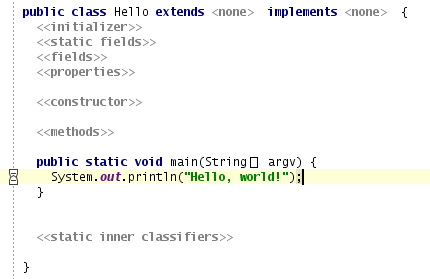
\includegraphics[width=0.9\textwidth]{ClassInMPS.png}
}
\caption{Редактор для класса в среде \MPS{}}
\label{fig:ClassInMPS}
\end{figure}

\section{Структура кода в среде \MPS{}}
Каждой конструкции программы в среде \MPS{} соответствует узел АСГ. Узел может содержать:
\begin{itemize}
 \item простые свойства, например, имя у переменной или значение у числовой константы;
 \item дочерние узлы, если в состав соответствующей конструкции входят другие конструкции, например, операнды бинарной операции;
 \item ссылки на другие узлы АСГ, например, узел, соответствующий использованию переменной, ссылается на узел, соответствующий декларации переменной.
\end{itemize}

Например, выражению "<i < 10"> соответствует фрагмент АСГ, представленный на рисунке \ref{fig:Less}.
\begin{figure}
 \centering
 \fbox{
  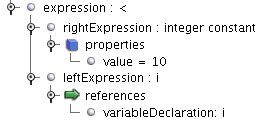
\includegraphics{Less.png}
 }
 \caption{Фрагмент АСГ, соответствующий выражению "<i < 10">}
 \label{fig:Less}
\end{figure}

Никуда не вложенные узлы называются корневыми. Корневые узлы соответствуют модулям-файлам в текстовых языках программирования. Каждый корневой узел вместе со всеми вложенными в него узлами принадлежит некоторой модели. Каждая модель, в свою очередь, принадлежит некоторому модулю. Модули бывают нескольких типов. Наиболее важными среди них являются решения (solution) и языки.

Решения представляют собой законченные программы или подсистемы программ, написанные с использованием различных языков, разработанных в среде \MPS{}.

Модели, входящие в состав языка, описывают различные аспекты этого языка: абстрактный и конкретный синтаксис, систему типов, операционную семантику и т.п. Следует отметить, что для описания всех этих аспектов также созданы проблемно-ориентированные языки, и, более того, применен принцип раскрутки, то есть эти языки переписаны уже при помощи самих себя.

Каждому типу языковых конструкций соответствует ровно одна декларация типа узла. Типы узлов в среде \MPS{} называются "<концептами">. Новый термин введен для того, чтобы отличать понятие для типа узла от понятий "<типа"> и "<класса">, которые имеют свой собственный смысл во многих языках программирования. Концепт узла, соответствующего некоторой конструкции, также является узлом и находится в специальной модели того языка, которому принадлежит эта конструкция. Например, концептом конструкции "<i < 10"> является корневой узел \term{LessThanExpression}, находящийся в модели \term{structure} языка \term{jetbrains.mps.baseLanguage} \pic{\ref{fig:LessThenExpressionConcept}}.

\begin{figure}
 \centering
 \fbox{ 
  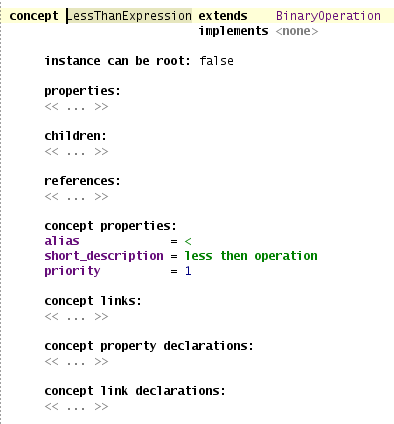
\includegraphics[width=0.7\textwidth]{LessThanExpressionConcept.png}
 }
 \caption{Концепт конструкции "<меньше">}
 \label{fig:LessThenExpressionConcept}
\end{figure}


Таким образом, на мета-уровне у узла может быть два типа ссылок: узел может ссылаться на другие узлы, как, например, "<использование переменной">, ссылается на "<декларацию переменной">; и узел является экземпляром некоторого концепта, как узел, соответствующий конструкции "<i < 10">, является экземпляром концепта \term{LessThanExpression}.

У каждой модели есть явно заданный набор используемых языков и набор импортированных моделей. Модель может содержать только те узлы, которые являются экземплярами концептов набора используемых ею языков.

Узлы могут ссылаться друг на друга внутри одной модели. Кроме того, узел из одной модели может ссылаться на узел из другой модели. Для этого вторая модель должна быть импортирована в первую.

Концепт в среде \MPS{} может иметь мета"=свойства и мета"=отношения, составляющие его мета"=структуру. Мета"=структура используется при описании аспектов языка, но не при программировании на нем.

\section{Поддержка Java-платформы в среде "<MPS">}
Ядро среды "<MPS"> написано на кросс-платформенном языке "<Java"> \cite{eckel}. В связи с этим в среде "<MPS"> существуют развитые средства для взаимодействия с Java-платформой. Для написания Java-кода в среде "<MPS"> разработан язык "<jetbrains.mps.baseLanguage"> (далее "<baseLanguage">). Этот язык является почти полной реализацией спецификации "<Java 5"> \cite{java5spec}. В нем определены такие концепты, как "<класс">, "<интерфейс">, "<метод">, "<предложение">, "<выражение"> и т.д.

Библиотеки, написанные непосредственно на языке "<Java">, могут быть использованы при разработке кода на языке "<baseLanguage">. Для этого среда "<MPS"> предоставляет доступ к пакетам библиотек, как к моделям. Классы, поля и методы из этих пакетов представляются экземплярами соответствующих концептов языка "<baseLanguage">.

Таким образом, для того, чтобы в своей модели написать на языке "<baseLanguage"> класс, выводящий на консоль сообщение "<Hello, world!">, необходимо добавить в набор, используемых моделью языков --- "<baseLanguage">, а в набор, импортированных моделей ---
"<java.lang@java\_stub"> и "<java.io@java\_stub">
(Рис. \ref{fig:Import}). Суффикс "<@java\_stub"> в именах моделей, указывает на то, что эти модели являются на самом деле пакетами языка "<Java">.
\begin{figure}
 \centering
 \fbox{
  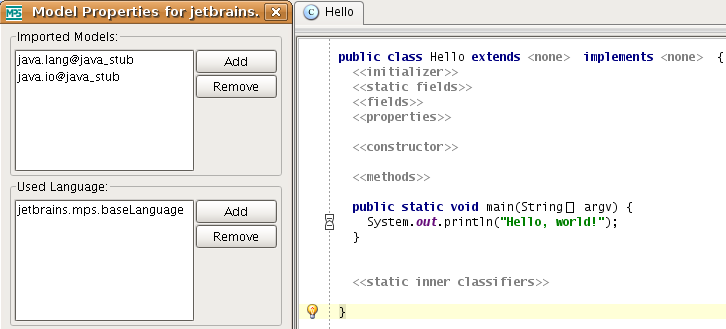
\includegraphics[width=\textwidth]{Import.png}
 }
 \caption{Код класса, выводящего на консоль строку «Hello, world!», и список используемых языков и импортированных моделей}
 \label{fig:Import}
\end{figure}

\section{Исполнение программ, разработанных в среде "<MPS">}
Для того, чтобы код, написанный в среде "<MPS">, можно было запустить, применяются интерпретационный, генерационный или смешанный подходы \cite{semantics}. Так как исходный код в среде "<MPS"> храниться непосредственно в виде АСГ, отпадает необходимость в лексическом и синтаксическом разборе кода и процессе разрешения ссылок. То есть исходный код сразу готов к интерпретации. Но интерпретационный подход обладает существенным недостатком: интепретация АСГ не может происходить вне среды "<MPS">, кроме того, интерпретация АСГ как правило менее эффективна, по сравнению с выполнением генерированного машинного кода.

Генерация в среде "<MPS"> использует индукционный подход. Базовым в этой индукции является язык, для которого написан текстовый генератор, который преобразует корневые узлы АСГ в текстовые файлы. Например, в среде "<MPS"> определен текстовый генератор для языка "<baseLanguage">, который генерирует код на языке Java. Текстовые генераторы просты по своей структуре, и фактически реализуют обход АСГ в глубину \cite{cormen} с выводом в файл соответствующего текста для каждого узла дерева.

Вместо текстового генератора для каждого концепта языка можно определить правила преобразования в концепты других языков. Таким образом осуществляется переход индукции. То есть для того, чтобы среда "<MPS"> могла преобразовать узел АСГ в текст, для этого узла должен быть либо определен текстовый генератор, либо правила преобразования в узел, который может быть преобразован в текст.

На момент написания данной работы среда "<MPS"> способна осуществлять генерацию только моделей целиком, используя при этом следующий алгоритм:
\newcounter{algorithmStep}
\newcommand{\algStep}[1]{\refstepcounter{algorithmStep}\label{alg:#1}}
\newcommand{\refStep}[1]{\ref{alg:#1}}
\begin{enumerate}
 \item \algStep{init}
Установить модель, которую необходимо преобразовать в текст, в качестве \textit{входной модели}.

 \item \algStep{loopStart}
Если ни для одного узла \textit{входной модели} не найдено ни одного правила преобразования в другой узел, перейти к шагу \refStep{textgen}.

 \item \algStep{reduce}
Создать \textit{целевую модель} и скопировать в нее все узлы \textit{входной модели}, при этом,  узлы, для которых найдены правила преобразования, заменить результатом применения этих правил.

 \item \algStep{loopEnd}
Установить полученную \textit{целевую модель} в качестве \textit{входной модели}, перейти к шагу \refStep{loopStart}.

 \item \algStep{textgen}
К каждому корневому узлу \textit{входной модели} применить текстовый генератор.
\end{enumerate}

Выполнению этого алгоритма могут помешать различные ошибки, допущенные при разработке генераторов. Во-первых, правила генерации могут быть написаны таким образом, что выходная модель всегда будет содержать узлы, для которых найдутся правила генерации. Чтобы это не приводило к зависанию генерации, в среде "<MPS"> наложено конечное ограничение на количество циклов генерации. То есть, если исходная модель не была преобразована в текст за некоторое конечное количество шагов, то генерация прекращается,  а пользователю выдается сообщение об ошибке.

Во-вторых, для некоторых корневых узлов входной модели, полученной к шагу \refStep{textgen}, может не существовать текстового генератора. Про каждый такой узел пользователю будет выдано сообщение об ошибке, но остальные узлы будут корректно преобразованы в текстовые файлы.

В-третьих, для некорневых узлов на шаге \refStep{textgen} может быть не определено правило преобразования в текст. В этом случае пользователю также будет выдано сообщение об ошибке, а вместо текста, соответствующего такому узлу, в файл будет выведено имя концепта узла.

В-четвертых, при вычислении правила генерации может произойти исключительная ситуация \cite{eckel}. Если это произойдет, генерация будет остановлена, а информация об исключительной ситуации выведена пользователю.


%%\TBD Язык smodelLanguage — расширение baseLanguage для манипулирования моделями
%%\TBD Язык collectionLanguage — функциональное расширение baseLanguage для работы с коллекциями
%%\TBD Язык quotation — расширение baseLanguage для создания фрагментов АСТ-дерева.

\section{Существующие автоматные языки}
Доминирующей в современном программировании является объектно-ориентированная парадигма программирования \cite{meyer}. При этом для описания поведения объектов, как правило, используется процедурный подход \cite{nepeyvoda}. Однако для целого ряда задач управления больше подходит автоматный подход \cite{shalyto01,shalyto02}. К настоящему моменту существует несколько языков, поддерживающих программирование автоматов, как в рамках автоматной парадигмы (UniMod FSML \cite{lagunov}, State Machine \cite{shamgunov}), так и вне ее (SMC \cite{smc}, ТАВР \cite{tsimbaluk}, SCXML \cite{scxml}, Ragel \cite{ragel}). Каждый из этих языков программирования обладает некоторыми недостатками и ограничениями.

Программирование в среде "<UniMod"> предполагает, что разработка ведется исключительно на базе автоматной парадигмы \cite{myUMLSwitchEclipse}. Это затрудняет использование среды "<UniMod"> в тех случаях, когда необходимо описать автоматное поведение класса, в программе, разрабатываемой в рамках традиционного объектно-ориентированного подхода.

Язык "<State Machine">, представляет собой расширение языка "<Java">, основанное на паттерне проектирования "<State Machine"> \cite{gof}. Этот паттерн позволяет в объектно-ориентированном стиле описывать структуру автомата, однако такое описание оказывается громоздким, что препятствует использованию языка "<State Machine"> в реальной разработке.

Язык "<SMC"> --- универсальный компилятор автоматов. Этот язык позволяет описывать в автоматы в едином формате и генерировать целевой код на различных языках общего назначения. Но интеграция этого языка с целевыми языками требует от разработчиков дополнительных усилий --- необходимо существенно модифицировать код класса для того, чтобы связать его с автоматом, описывающим его поведение.

В универсальном языке программирования "<ТАВР"> предусмотрены встроенные конструкции, облегчающие написание автоматов. Однако синтаксис этого языка вынуждает разработчика оперировать понятиями более низкоуровневыми, чем "<состояние">. Кроме того, универсальность языка "<ТАВР"> доставляет дополнительные трудности разработчику, связанные с необходимостью изучать конструкции нового языка даже для тех задач, для которых подходят более распространенные универсальные языки.

Язык "<Ragel"> предназначен для описания конечных автоматы с помощью регулярных выражений. Такой подход ограничивает область применимости этого языка задачами лексического анализа и спецификации протоколов,

Стандарт языка "<SCXML"> --- спецификация XML-представления автоматов Харела \cite{harel}. Использовать этот язык непосредственно для написания кода автоматов на нем крайне затруднительно, скорее он подходит для обмена автоматами Харела между приложениям.

Существуют и другие языки так или иначе позволяющие использовать автоматы при программировании. Что доказывает популярность автоматного подхода для решения различных задач программирования. В связи с этим, процесс создания языка в среде "<MPS"> будет продемонстрирован на примере языка "<jetbrains.mps.baseLanguage.stateMachine">, являющегося автоматным расширением языка "<baseLanguage">.

\section{Язык \term{jet\-bra\-ins.mps.ba\-se\-Lan\-gu\-age.sta\-te\-Ma\-ch\-ine}}
Проблемно"=ориентированный язык \term{jet\-bra\-ins.mps.ba\-se\-Lan\-gu\-age.sta\-te\-Ma\-chi\-ne} (далее \term{stateMachine})
представляет собой автоматное расширение языка \term{baseLanguage}. Основная цель, которая приследовалась при разработке
языка \term{stateMachine}, --- создать средство, позволяющее описывать поведение классов в виде автоматов, не накладывая на
сами классы никаких дополнительных ограничений. Более того, автоматное описание поведения класса должно быть
инкапсулировано. То есть код, использующий класс не должен "<знать"> о том, каким образом задано поведение класса. Этот
подход отличается от предложенного в работе \cite{myUMLSwitchEclipse} тем, что позволяет использовать автоматы не только в
программах написанных в соответствии со SWITCH-технологией, но и в традиционных объектно-ориентированных программах.

В качестве примера использования языка \term{stateMachine} взята система управления лифтом \cite{knuth}. Используемая
реализация системы является упрощенным решением задачи управления лифтом, описанном в работе \cite{naumov}. Логика
управления всеми подсистемами лифта реализована в одном автомате.

Каждый автомат в языке \term{stateMachine} связан с некторым классом и описывает его поведение. Для удобства редактирования
автомат описывается в отдельном корневом узле \pic{\ref{fig:ElevatorStateMachine}}.

\begin{figure}
 \centering
 \fbox{
  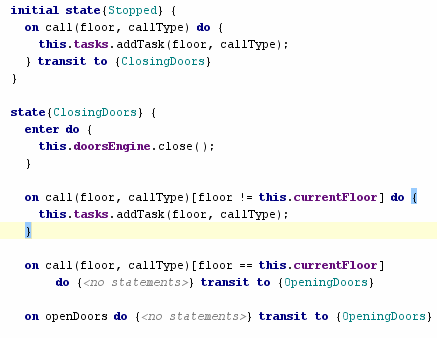
\includegraphics[width=0.7\textwidth]{ElevatorStateMachine.png}
 }
 \caption{Фрагмент автомата управляющего лифтом}
 \label{fig:ElevatorStateMachine}
\end{figure}

Для того чтобы задать поведение класса с помощью автомата в языке \term{stateMachine} необходимо в этом классе определить
события, на которые будет реагировать автомат. Особенностью языка \term{stateMachine} является то, что события в нем --- это
методы специального вида. В языке \term{Java} декларации методов различаются по способу реализации:
\begin{itemize}
 \item обычные методы, реализация которых следует сразу за объявлением метода;
 \item нативные методы, реализованные на платформо-зависимых языках программирования;
 \item абстрактные методы, вообще не имеющие реализации.
\end{itemize}
Событие в языке \term{stateMachine} --- это метод, реализация которого находится в автомате и зависит от текущего состояния
автомата. Например, в классе \term{Elevator} объявлены следующие события \pic{\ref{fig:ElevatorEvents}}
\begin{description}
 \item[doorsOpened, doorsClosed] --- события, которые посылает объект управления \term{DoorsEngine}, когда двери оказываются в максимально открытом и полностью закрытом положении соответственно;
 \item[floorReached] --- событие, которое посылает объект управления \term{ElevatorEngine}, когда лифт достигает очередного этажа;
 \item[call] --- событие, которое получает автомат, когда пассажир нажимает кнопку вызова лифта на этаже, или в кабине лифта;
 \item[openDoors] --- событие, которое получает автомат, когда пассажир нажимает кнопку экстренного открывания дверей в кабине лифта;
 \item[loadingTimeout] --- событие, которое посылает объект управления \term{LoadingTimer}, когда истекает время ожидания погрузки пассажиров.
\end{description}
\begin{figure}
 \centering
 \fbox{
  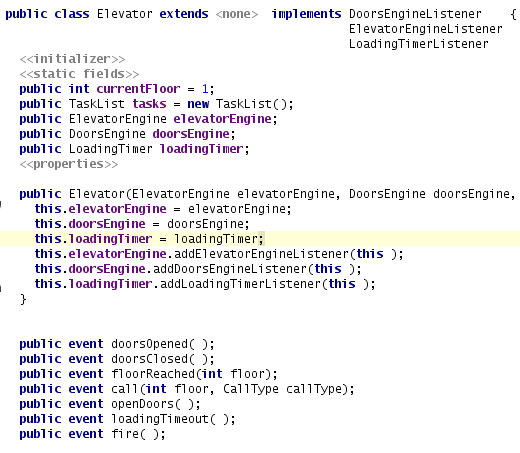
\includegraphics[width=0.9\textwidth]{ElevatorEvents.png}
 }
 \caption{События автомата управляющего лифтом}
 \label{fig:ElevatorEvents}
\end{figure}
Так как события являются обычными методами, их можно использовать в качестве реализации абстрактных методов. Это позволяет
уменьшить количество зависимостей в программе. Например, объект управления \term{ElevatorEngine} не имеет непосредственных
ссылок на класс \term{Elevator}. Вместо этого в программе объявлен интерфейс \term{ElevatorEngineListener}, и объект
управления \term{ElevatorEngine} извещает о событиях экземпляры этого интерфейса. Класс \term{Elevator} реализует интерфейс
\term{ElevatorEngineListener} и поэтому может обрабатывать события объекта управления \term{ElevatorEngine}. Таким образом
удается классически реализовать паттерн проектирования \term{Обозреватель} \cite{gof}.

Реакция автомата на событие зависит от состояния, в котором автомат находится. Состояния автомата бывают двух типов: обычные
и конечные. Конечные состояния отличаются тем, что не могут иметь исходящих переходов. То есть, когда автомат оказывается в
конечном состоянии он перестает обрабатывать события.

Первое состояние, объявленное в автомате, считается начальным. При создании экземпляра класса, для которого определен
автомат, после выполнения конструктора осуществляется переход в начальное состояние.

Обычные состояния могут быть вложены друг в друга. При этом, если состояние содержит

События, как и другие методы, могут иметь формальные параметры. Значения этих параметров доступны в условиях и действиях на
переходах.



Каждый автомат в языке \term{stateMachine} связан с некоторым классом, имеет доступ к полям и может вызывать методы этого
класса. Поэтому в языке \term{stateMachine} нет необходимости в специальных конструкциях для взаимодействия между
автоматами, так как вместо вложения одного автомата в другой можно использовать агрегацию одного класса с автоматом, другим
классом с автоматом, а посылка события из одного автомата в другой ни что иное как вызов метода.
\subsection{Абстрактный синтаксис}
Описание языка в среде \MPS{} обычно начинается с задания абстрактного синтаксиса \cite{redDragon} этого языка. Для этого в
среде \MPS{} предусмотрен специальный проблемно"=ориентированный язык \term{jet\-bra\-ins.mps.boot\-strap.struc\-tu\-re\-Lan\-ga\-uge} (далее
\term{structureLanguage}). Этот язык позволяет описать концепты языка и отношения между ними. С помощью этого же языка
задаются свойства и мета"=свойства концептов. Весь абстрактный синтаксис языка описывается в модели \term{structure} этого
языка.

Для объявления пользовательских концептов в языке \term{structureLangauge} определен концепт \term{ConceptDeclaration}.
Например, корневой узел, описывающий концепт \term{StateMachine}, предствлен на рисунке \ref{fig:StateMachineConcept}.

\begin{figure}
\centering
\fbox{
 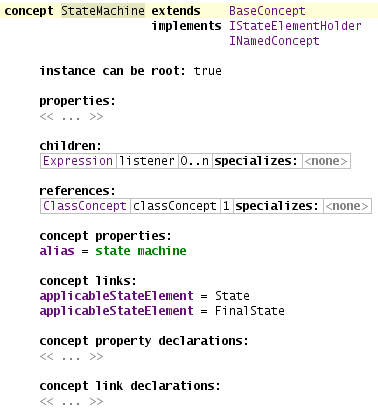
\includegraphics[width=0.9\textwidth]{StateMachineConcept.png}
}
\caption{Объявление концепта \term{StateMachine}}
\label{fig:StateMachineConcept}
\end{figure}


Из рисунка видно, что объявление концепта состоит из нескольких секций:
\begin{itemize}
 \item секция \term{concept StateMachine} задает имя концепта;

 \item секция \term{extends BaseConcept} указывает на то, что концепт является расширением концепта \term{BaseConcept}.
 Отношение расширения в языке \term{structureLanguage} имеет тот же смысл, что и в традиционных объектно"=ориентированных
 языках программирования: если концепт \term{B} является расширением концепта \term{A}, то все экземпляры концепта \term{B}
 являются также и экземплярами концепта \term{A}. Так же концепт \term{B} наследует все свойства и отношения концепта
 \term{A}.  Каждый концепт объявленный в среде \MPS{} является прямым или косвенным расширением концепта
 \term{BaseConcept},  также как в языке \term{Java} все классы прямо или косвенно расширяют класс \term{java.lang.Object};

 \item в секции \term{implements IStateElementHolder INamedConcept} перечислены интерфейсы"=концепты реализуемые
 концептом \term{StateMachine}. Понятие \term{интерфейса"=концепта} ближе всего к понятию \term{trait} языка \term{Scala} [ссылка].
 Интерфейс"=концепт также может иметь свойства и отношения с другими концептами. При этом не может быть узлов,
 являющихся непосредственными экземплярами интерфейса"=концепта. Интерфейсы"=концепты полезны для создания неполного
 множественного наследования: концепт наследует все свойства и отношения тех интерфейсов"=концептов, которые он
 реализует;

 \item в секции \term{instance can be root} задается могут ли экземпляры концепта быть корневыми узлами моделях. В
 данном случае, экземпляры концепта \term{StateMachine} могут быть корневыми;

 \item в секции \term{properties} перечисляются свойства, которые может иметь экземпляр концепта. Концепт 
\term{StateMachine} не определяет собственных свойств, однако у экземпляров этого концепта может быть задано свойство 
\term{name}, унаследованное от интерфейса"=концепта \term{INamedConcept};

 \item в секции \term{children} описывается структура вложенных узлов. Для каждого элемента в этой секции задается концепт,
роль и арность вкладываемых узлов. Арность определяет ограничение на количество вложенных экземпляров данного концепта с
данной ролью. Арность может быть задана одним из четырех значений:
\begin{description}
 \item["<1">] ровно один экземпляр;
 \item["<0..1">] не более одного экземпляра;
 \item["<1..n">] хотя бы один экземпляр;
 \item["<0..n">] произвольное количество экземпляров.
\end{description}
Например, в экземпляр концепта \term{StateMachine} может быть вложено произвольное количество экземпляров концепта 
\term{Expression} с ролью \term{listener}. Кроме этого экземпляр концепта \term{StateMachine} может содержать произвольное
количество вложенных экземпляров интерфеса"=концепта \term{IStateElement}, так как в секции \term{children}
интерфейса"=концепта \term{IStateElementHolder} есть элемент \term{IStateElement stateElement 0..n}, и концепт 
\term{StateMachine} реализует интерфейс"=концепт \term{IStateElementHolder};

\item в секции \term{references} определяется структура ссылок концепта. Также, как и в случае вложенных узлов, каждый
элемент в этой секции задает целевой концепт, роль и арность ссылки. Арность ссылки может быть задана одним из двух значений:
\begin{description}
 \item["<1">] обязательная ссылка;
 \item["<0..1">] необязательная ссылка.
\end{description}
Например, каждый экземпляр концепта \term{StateMachine} должен иметь ссылку с ролью \term{classConcept} на экземпляр
концепта \term{ClassConcept};

\item четыре последних секции предназначены для описания мета"=структуры концепта. в секции \term{concept properties} задаются
значения мета"=свойства концепта. Для концепта \term{StateMachine} значение мета"=свойства \term{alias} определено как 
\term{state machine}. Это специальное мета"=свойство, значение которого используется средой \MPS{} в качестве имени концепта
в пользовательском интерфейсе. Например, в меню создания корневого узла, опция, соответствующая созданию экземпляра концепта
\term{StateMachine}, будет называться \term{state machine} (Рис. \ref{fig:CreateStateMachine}).

\begin{figure}
 \centering
 \fbox{
  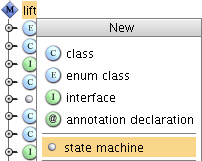
\includegraphics{CreateStateMachine.png}
 }
 \caption{Меню создания корневого узла}
 \label{fig:CreateStateMachine}
\end{figure}

В секции \term{concept links} задаются значения мета"=отношений концепта. В секциях \term{concept property declaration} и
\term{concept link declarations} объявляются мета"=свойства, значения которых могут быть заданы в самом концепте или в
расширяющих его концептах. Например, в интерфейсе"=концепте \term{IStateElementHolder} объявлено мета"=отношение 
\term{applic\-able\-Sta\-te\-Ele\-ment}, значение которого используется в языке \term{stateMachine} для того, чтобы уточнить
какие именно автоматные конструкции могут быть вложены в другие автоматные конструкции. Значения
$$
\begin{array}{l}
applicableStateElement = State\\
applicableStateElement = FinalState
\end{array}
$$
для концепта \term{StateMachine} указывают на то, что автомат может содержать обычные и конечные состояния.
\end{itemize}

Абстрактный синтаксис языка может быть представлен виде UML"=диаграммы классов \cite{uml}. Для языка \term{stateMachine}
такая диаграмма приведена на рисунке \ref{fig:AbstractSyntax}.

\begin{figure}
 \centering
 \fbox{
  
\includegraphics[angle=90,width=0.9\textwidth]{AbstractSyntax.png}
 }
 \caption{Абстрактный синтаксис языка \term{stateMachine}}
 \label{fig:AbstractSyntax}
\end{figure}

\subsection{Конкретный синтаксис}
Для задания конкретного синтаксиса в среде \MPS{} предусмотрен проблемно"=ориентированный язык \term{jet\-bra\-ins.mps.lang.ed\-it\-or}. Он позволяет для каждого концепта определить редактор, описывающий представление узлов этого концепта в виде набора ячеек. Каждая ячейка редактора соответствует ключевому слову, свойству, вложенному узлу, ссылке или другому члену концепта. Например, для концепта \term{StateMachine} определение редактора приведено на рисунке \ref{fig:StateMachineEditor}.

\begin{figure}
 \centering
 \fbox{
  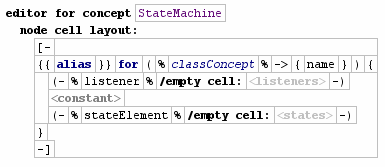
\includegraphics[width=0.9\textwidth]{StateMachineEditor.png}
 }
 \caption{Редактор для концепта \term{StateMachine}}
 \label{fig:StateMachineEditor}
\end{figure}

\begin{enumerate}
\item Конструкция "<[- ... -]"> --- составная ячейка. Она используется для того, чтобы задать конкретное представление узла концепта \term{StateMachine} в виде набора ячеек. В этом представлении никакой текст для нее выводиться не будет.
\item Ячейка "<\{\{alias\}\}"> соответствует мета"=свойству \term{alias} концепта \term{StateMachine}. Значением этого мета"=свойства, как было указано ранее, является строка "<state machine">. Таким образом, конкретное представление узлов концепта \term{StateMachine} начинается с ключевого слова "<state machine">. Для каждой ячейки 
\MPS{}"=редактора можно задать стиль. В частности, для первой ячейки задан стиль ключевого слова из языка \term{baseLanguage}.
\item В ячейке "<for"> указан текст, который будет безусловно выводиться на второй позиции.
\item Ячейка "<(\%classConcept\% -> \{name\})"> описывает представление ссылки с ролью \term{classConcept}. Вложенная ячейка "<\{name\}"> определяет то, что в качестве представления ссылки будет использовано значение свойства \term{name} того узла, на который указывает ссылка.
\item Ячейка "<\{"> соответствует открывающейся фигурной скобке.
\item Ячейка "<(-\%listener\% /empty cell: <listeners>-)"> соответствует вложенным узлам с ролью \term{listener}. На место этой ячейки будут вставлены конкретные представления вложенных узлов. Причем для каждого вложенного узла будет использован соответствующий его концепту редактор. Если у некоторого данного узла \term{StateMachine} нет вложенных узлов с ролью \term{listener}, то будет выведен текст "<<listeners>">.
\item Ячейка "<<constant>"> --- пустая ячейка без текста, в данном случае она соответствует пустой строке.
\item Ячейка "<(-\%stateElement\% /empty cell: <states>-)"> аналогично соответствует вложенным узлам с ролью 
\term{stateElement}.
\item Ячейка "<\}"> --- закрывающаяся фигурная скобка.
\end{enumerate}

На рисунке \ref{fig:EmptyStateMachine} приведен пример конкретного представления узла концепта \term{stateMachine} с двумя состояниями. Данный узел описывает автоматное поведение класса \term{SomeStatefulClass}. Узлы, соответствующие его состояниям, имеют роль \term{stateElement}.

\begin{figure}
 \centering
 \fbox{
  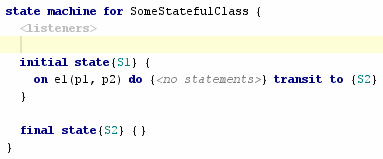
\includegraphics[width=0.9\textwidth]{EmptyStateMachine.png}
 }
 \caption{Представление узла концепта \term{stateMachine} с двумя состояниями}
 \label{fig:EmptyStateMachine}
\end{figure}

\subsection{Несинтаксические ограничения модели}


\bibliography{languages}

\end{document}
